\chapter{Notes for the Password Cracking Assignment}

One of the things we want to focus on this class is the idea of thinking about security in a systematic way. This means to try to think about it in a repeatable and almost formal way. How can we do this for the problem of password cracking? 

Well let’s think of a model for password cracking.

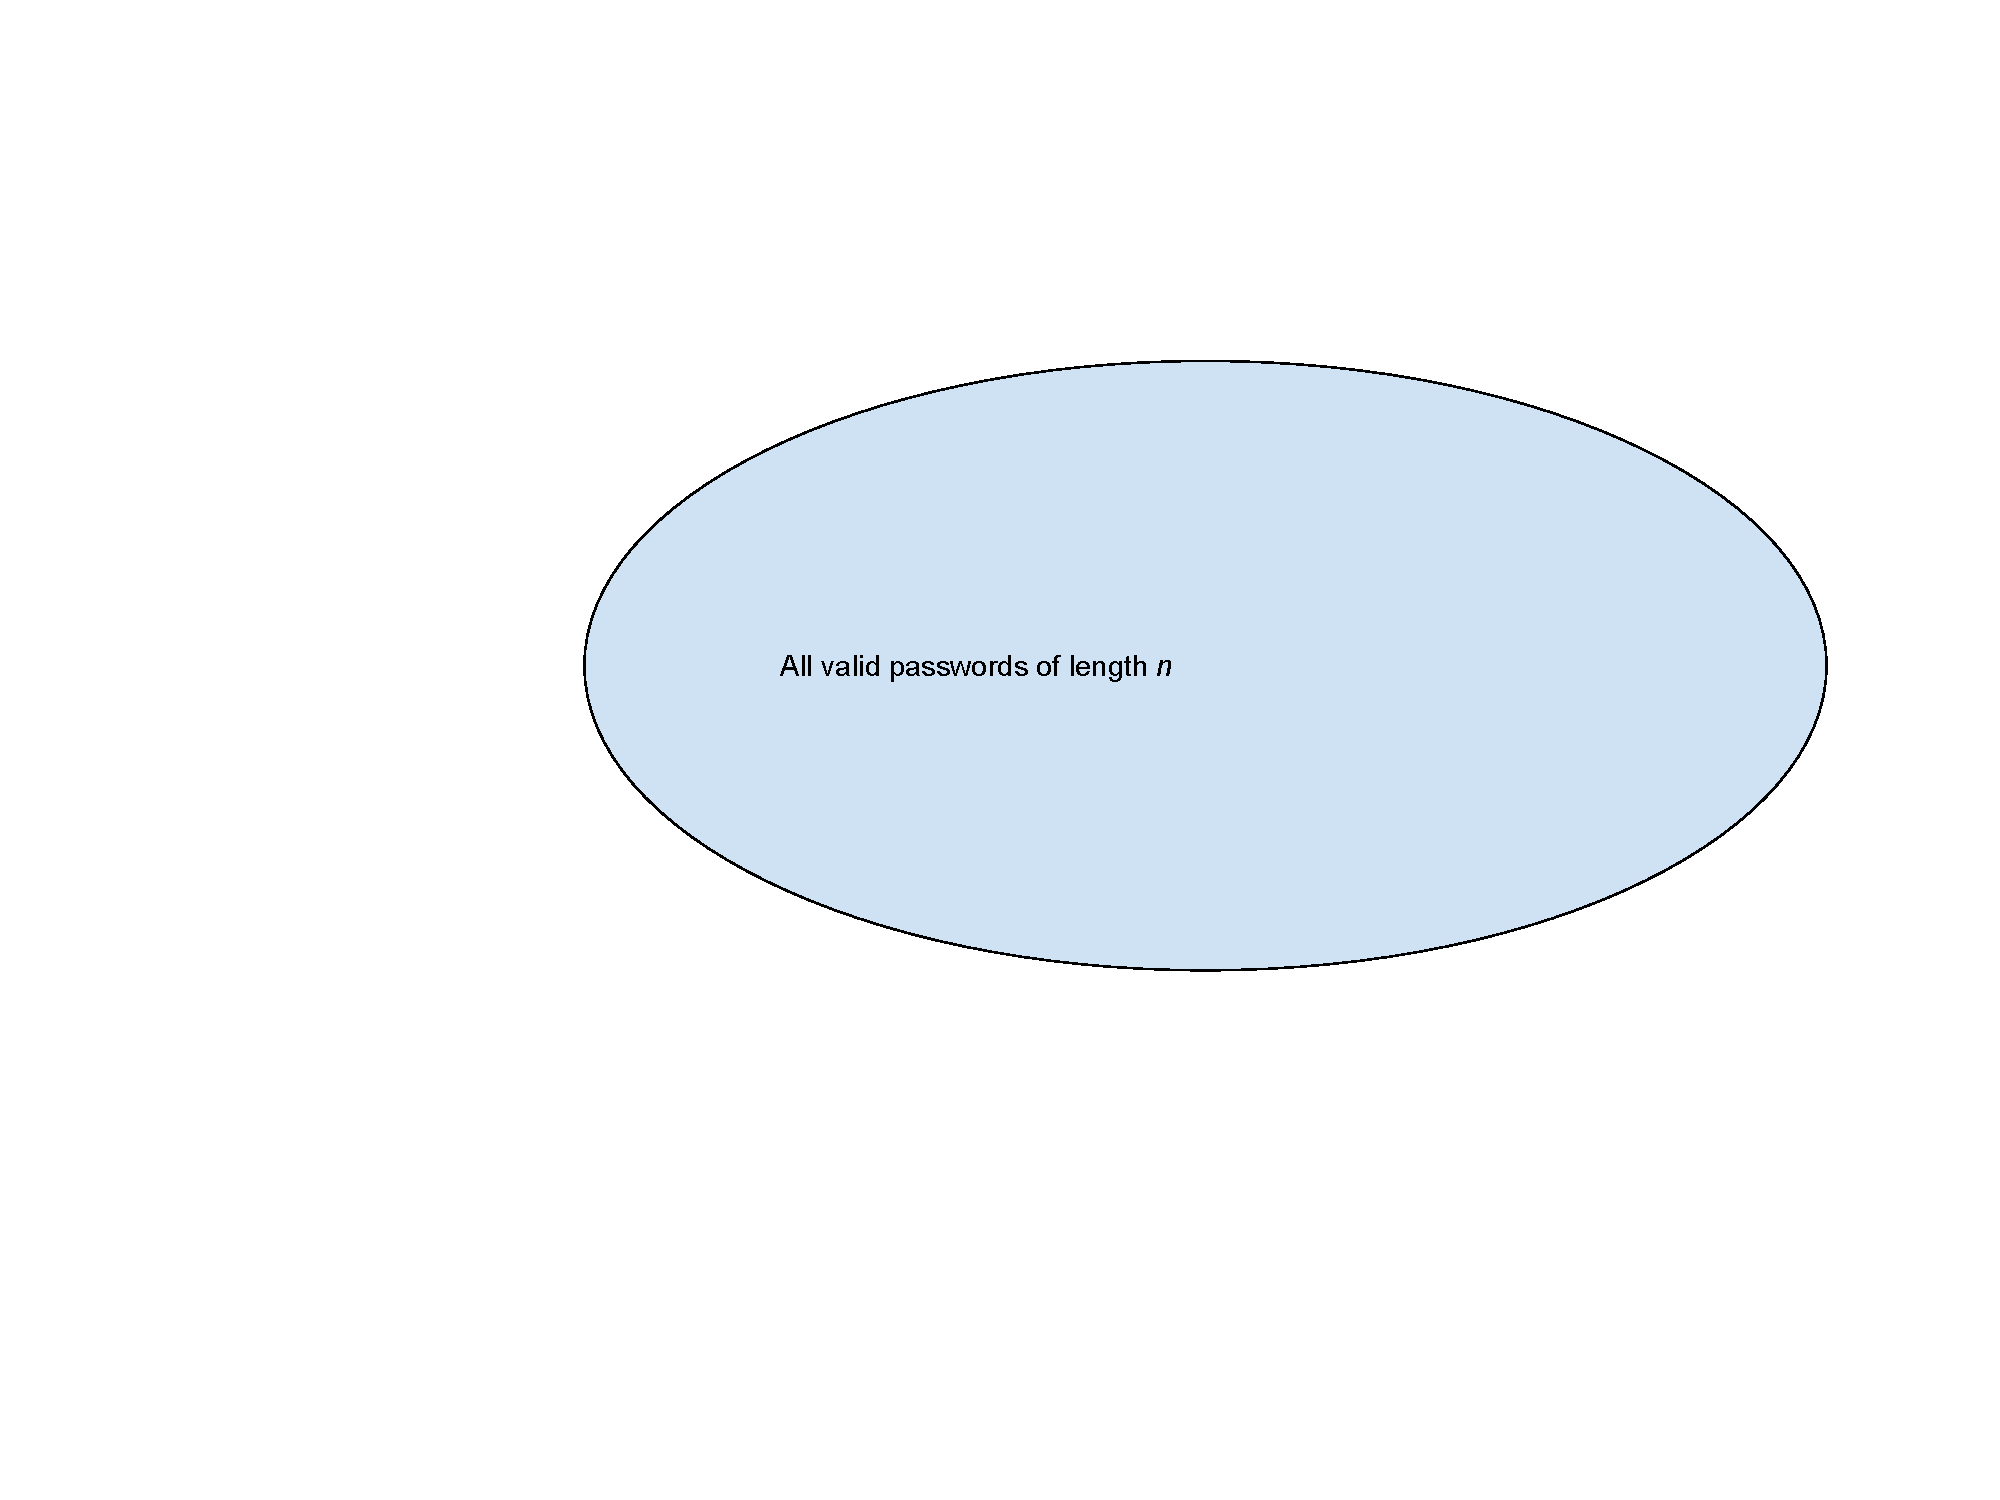
\includegraphics[width=5in]{Assignments/images/PasswordCracking_1}

If we think of what a “password” is, then we know that a password is just a series of ‘characters’ of a certain length. This seems like a set type of problem, meaning we will try to reason about this in a Venn diagram.

Now that we have the big giant set, let’s start thinking about different subsets such as the subset of all passwords of a lesser length (note the use of “up to”)

Let us also include other subsets.

Now that we have a good idea, let’s start thinking about the process of password cracking. First is the dictionary attack that consists of only English words. Note that instead of “dictionary” it is best to think of this type of attack as a “wordlist” since a dictionary is a list of words, but there can be other lists that aren’t made up of real words that might appear in a dictionary in the traditional sense. Either way, this is a very nice attack since it fits in directly over the set of passwords that are simply “English words of length up to n.”

What about our second approach that uses a dictionary of previously cracked passwords?

Now if we think about this a bit more, we might notice that each successive dictionary or wordlist is represented by yet another sub-set. The same applies to perturbations to the wordlists - such as prepending 2 numbers in front of the wordlist to generate the ‘salted’ passwords in formspring.

If you then think about all of the wordlists and perturbation rules (called ‘masking’ in hashcat or ‘mangling’ in John the Ripper) then we might see a venn diagram such as the one below. We can also clearly see that the goal of choosing a ‘good’ password is to choose one that is not covered in any of the sub-sets (look for the ‘X’)

Okay, now given this, let’s talk about the ‘brute force’ mode. The idea of ‘brute’ force is to tray all possible combinations, which means we want the entire set. This obviously covers the ‘X’ meaning it will recover ANY password chosen from the set.

While this is problematic from a theoretical point of view, we also quickly realize that while we can cover the entire space, we can’t do it all at once. We have to do it step by step. One such way is to simply iterate through all possible combinations linearly as depicted by the arrows. It will takes a while to get to the X using our current trajectory that goes from left to right and top to bottom (whatever that might mean). It might be faster to go down and up and then left to right (whatever that means).

The above diagram is how most people think of ‘brute force’. A dumb way of simply iterating through the space. However, note that we defined ‘brute force’ as trying all possible combinations. The how we traverse through this space is part of the ‘strategy’ for brute forcing. What is a better strategy? What about one that starts with the dictionary or wordlist attacks first? Followed by previously cracked passwords followed by perterbations on them? The following diagram should look familiar.

What I want you to see here is basically that wordlist or dictionary attacks should simply be thought of as the first stages of a ‘brute force’ attack because it is a subset. It should be part of your strategy. Furthermore, I want you to see that the strategy for choosing a ‘good’ password does not change much. Instead of saying that we want to choose a password ‘X’ that is outside of the wordlists, we are basically saying that we want to choose a password ‘X’ that will not be covered by the first m stages of a prioritized brute force attack. A good rule of thumb is where m is big enough so that it will take an attacker a certain amount of time to crack - e.g. one year’s time. This naturally means that it must not be part of any wordlist attack!
One way to calculate how long it might take for an attacker to crack your password is by assuming that the attacker will use a “random” strategy where passwords to try are chosen randomly from the set of passwords that haven’t been tried yet (the light blue in the diagram above since the yellow parts have already been tried). The random guess is a very common technique. This is the source of a common password policy which is to use randomly generated passwords - good for security, but bad when it comes to the principle of psychological acceptability.
One approach to reduce the likelihood of an attacker guessing your password within that 1 year time frame (or however long you desire) is to increase the size of the light-blue space without increasing the size of the wordlists, meaning there will be so many more possible possible passwords within the non-wordlist set that randomly guessing the password will cover a smaller portion of the overall space and therefore result in a less likelihood of having your password. This is the same fundamental idea behind the increase in key-sizes in cryptographic algorithms. Graphically it looks like this. This is one way to reason about why it makes sense to use “passphrases” versus “passwords” because passphrases, while they are made up of dictionary words, are so long that the likelihood of guessing the new password is very low.

It should be clear that another way to decrease the likelihood of success is to increase the time it takes to calculate the hash. This reduces the number of possible passwords attackers can try within that 1 year timeframe (or however long you want). This is why you might want to use bcrypt instead of sha256 for example.
One thing we didn’t discuss here is the concept of pre-calculated hashes known as a rainbow-table attack. (Note that because we focus on the fundamental concepts in this course, the definition of rainbow-table is a ‘pre-calculated table of hashes’ versus what you might find online which normally consists of a specially designed hash tree structure.). It is actually a different dimension that isn’t calculated here, but it is interesting for you to consider.
FInally, it might also be interesting to think about how “salting” passwords can either increase or decrease the likelihood of finding the password. One way of thinking about this is by relating “salting” to mangling rules. This should give you some insights into how much does salting help. Ask yourself if the simple salt used in Formspring really made dictionary attacks that much more difficult? Did it really only increase the size of the dictionary by 100 fold?

